\documentclass[12pt]{article}
\usepackage{amsmath}
\usepackage{graphicx}
\usepackage{float}

%\setlength\parindent{20pt} %% Do not touch this

\title{Analytic Tools for the Finite Element Method on Parabolic Equations} 

\author{Geneva Porter, SDSU Spring 2020\\ 
Numerical Partial Differential Equations\\
Dr. Uduak George, Applied Mathematics}

\date{7 May, 2020} 
\begin{document}
\maketitle

The finite element method (FEM) is a technique used to solve many different types of partial differential equations on a variety of meshes. Almost always implemented numerically, the FEM has several practical applications in applied mathematics. This report will detail one particular application, solving a parabolic reaction-diffusion equation on a surface geometry, and discuss ways in which the theoretical application is valid. Then, we will compare the analytic solution on the surface of a sphere with a solution using the FEM. The proceeding error analysis will examine to solution L2 and H1 norms, as well as the difference when mesh density changes.

\section{The Finite Element Method}

Notes to add to thesis: add details from short explanation on FEM from "Stability, consistency, and convergence" by D Arnold.

\section{Theoretical Validation/Convergence}

\section{Analytic vs. Numeric Comparison}

\pagebreak


\section{Error Analysis}

\subsection{Mesh Refinement and Convergence}

To examine how the choice of a mesh domain influences the convergence of the system, we examined 4 separate spherical surfaces of varying density. The sphere with the lowest density contained 96 quadrilateral cells on a spherical surface of unit-less radius 1. The next contained 384 cells, then 1,536, and finally 6,144. Note that each mesh was refined by a factor of 4, as each quadrilateral cell was sub-divided into 4 smaller cells with approximately half of their starting width. In this context, "width" is defined as the longest distance between two vertices n a single cell, and for these meshes, width always refers to the longest diagonal of the quadrilateral. 

After computing both the numeric solution using the FEM and the approximate analytic solution, we have a basis for testing our analysis. First, we can examine the convergence behavior for the four spheres from the numeric and analytic solutions. Figure \ref{fig:inner_norms} shows the convergence measure norms for $u$, given by:

$$ ||u||_C = \sqrt{\sum_n (u_{n} - u_{n+1})^2} $$

This measure is useful because it informs us about the behavior of the system over time. When the difference between terms becomes constant, we know that the system has reached an oscillatory steady state. Such behavior is typical for reaction-diffusion problems, particularly those with biochemical applications. 

\begin{figure}[H]
	
\includegraphics[width=.5\linewidth]{xxx.png}\\
	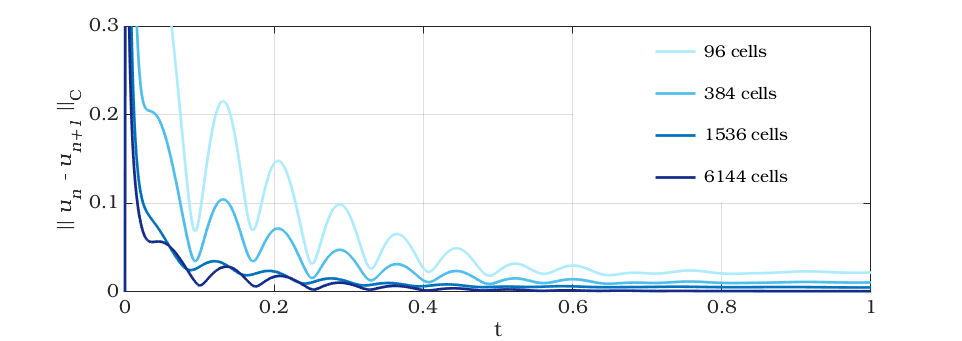
\includegraphics[width=\linewidth, trim= 1.4cm 0 2cm 0, clip]{norm_numeric.png}
	\caption{The convergence measure norms for the analytic solution (top) and the numeric solution (bottom) of the Schnakenberg system on a sphere.}
	\label{fig:inner_norms}
\end{figure}

Notice Figure \ref{fig:inner_norms} shows that for the numeric solutions, higher mesh density equates to a more stable convergence measure. In fact, as the width of the cells on the mesh halves, the value of the norm equilibrium halves as well. This is consistent with our previous findings, specifically Equation \ref{eq:error_cells}.

\section{Conclusion}

\end{document}













